% =============================================================================
\bloco{2}{Labor supply, taxes, transfers and search}{Kurlat ch.~7; Romer ch.~10 \,\textbullet\, 25 points}

\questao{(10 points) Objective items.}

\textbf{a)} (3 points) \emph{Labor $\times$ consumption smoothing.} A household lives $N\ge2$ periods with per-period utility
$\ln c_t-\psi\,h_t^{1+1/\varepsilon}/(1+1/\varepsilon)$, $\psi,\varepsilon>0$; it has no initial wealth, $\beta=1$ and $r=0$, and the wage is the same in every
period. The wage rises by the same small proportion in $k$ of the periods, $1\le k<N$. To first order, the elasticity of hours in a
period with the raise with respect to its wage is:
\begin{alternativas}
\item $\varepsilon$
\item $\varepsilon/(1+\varepsilon)$
\item $\varepsilon\,(N-k)/N$
\item $\varepsilon\,(N-k)/(N+k\varepsilon)$
\end{alternativas}
\gabarito{C}
\begin{sol}
\passo{FOCs}{With $\beta(1+r)=1$ the Euler equation gives $c_t=c$ in every period, and the hours condition $\psi h_t^{1/\varepsilon}=w_t/c$ gives
$d\ln h_t=\varepsilon\,(d\ln w_t-d\ln c)$.}
\passo{budget}{$Nc=\sum_tw_th_t$. At equal wages each period earns the share $1/N$, so $d\ln c=\frac1N\sum_t(d\ln w_t+d\ln h_t)$. Substituting the
FOC, $(1+\varepsilon)\,d\ln c=(1+\varepsilon)\frac kN\,d\ln w$, so $d\ln c=\frac kN\,d\ln w$ (the wealth effect is the share of earnings the raise touches): hours rise by
$\varepsilon\frac{N-k}{N}\,d\ln w$ in a raised period and fall by $\varepsilon\frac kN\,d\ln w$ in the others.}
\passo{distractors}{A holds the marginal utility of wealth fixed (pure Frisch response); B is the static compensated elasticity of these
preferences, with no intertemporal margin; D keeps only the raised periods' hours in the budget. A permanent raise ($k=N$) gives $0$:
log utility then cancels income and substitution effects.}
\refbib{Kurlat (2020), \S7.4, and Exercise 7.5(j)--(k) for the Frisch elasticity.}
\end{sol}

\medskip
\textbf{b)} (3 points) \emph{Search $\times$ wage setting.} Steady-state search model with matches $M=A_mU^{\xi}V^{1-\xi}$, $\xi\in(0,1)$, tightness
$\theta=V/U$, vacancy-filling rate $q(\theta)=M/V$ and free entry $(y-w)\,q(\theta)=(r+s)\kappa$, with $r,s,\kappa>0$. The wage is rigid at $w\in(0,y)$
while productivity $y$ moves. The elasticity of $\theta$ with respect to $y$ is:
\begin{alternativas}
\item $\frac{1}{\xi}\,\frac{y}{y-w}$
\item $\frac{1}{1-\xi}\,\frac{y}{y-w}$
\item $\frac{1}{1-\xi}$
\item $\frac{1-\xi}{\xi}\,\frac{y}{y-w}$
\end{alternativas}
\gabarito{A}
\begin{sol}
\passo{matching}{$q(\theta)=A_mU^{\xi}V^{-\xi}=A_m\theta^{-\xi}$ and $f=\theta q=A_m\theta^{1-\xi}$, so free entry reads $\ln(y-w)-\xi\ln\theta=\ln\frac{(r+s)\kappa}{A_m}$.}
\passo{log-differentiate}{With $w$ fixed, $\frac{y}{y-w}\,d\ln y=\xi\,d\ln\theta$, so $\frac{d\ln\theta}{d\ln y}=\frac1\xi\,\frac{y}{y-w}$: through the profit $y-w$ a rigid wage
amplifies $y$ by $\frac{y}{y-w}>1$ (one answer to Shimer's puzzle). B uses $1-\xi$, the elasticity of $f$, for that of $q$; C makes two
mistakes: it uses $1-\xi$ for $\xi$, as B does, and lets $w$ move in proportion to $y$, removing the amplification; D is the elasticity of $f$, $(1-\xi)\,d\ln\theta/d\ln y$.}
\refbib{Kurlat (2020), \S7.5; Romer (2012), \S10.6 and problem 10.15.}
\end{sol}

\medskip
\textbf{c)} (2 points, T or F) \emph{Search $\times$ efficiency.} One-shot matching: $U$ unemployed workers and $V$ vacancies, each costing
$\kappa>0$ to open (free entry), form $M(U,V)$ matches, with $M$ of constant returns, increasing and strictly concave in $V$. A match
produces $y$, of which the worker gets the share $\phi\in(0,1)$. The equilibrium maximizes net output $yM(U,V)-\kappa V$ if and only if $\phi$
equals the elasticity of $M$ with respect to $U$ at the equilibrium tightness.
\gabarito{T}
\begin{sol}
\passo{two conditions}{With $\theta=V/U$, $m(\theta)=M(1,\theta)$ and $q=m/\theta$, free entry is $(1-\phi)\,y\,q(\theta^e)=\kappa$; the planner's
$W(V)=yU\,m(V/U)-\kappa V$ is strictly concave, maximized at the unique root of $W'(V)=y\,m'(\theta)-\kappa$.}
\passo{wedge}{With $\eta_V\equiv\theta m'/m$, $m'=\eta_Vq$, and free entry gives $W'(V^e)=y\,q(\theta^e)\,[\eta_V(\theta^e)-(1-\phi)]$: $V^e$ is efficient iff
$\eta_V(\theta^e)=1-\phi$ (too many vacancies if $1-\phi>\eta_V$).}
\passo{constant returns}{Euler's theorem, $UM_U+VM_V=M$, gives $\eta_U=1-\eta_V$: the condition is $\phi=\eta_U(\theta^e)$, \textbf{True}. With returns
of degree $d\ne1$, $\eta_U+\eta_V=d$ and only the vacancy version holds.}
\refbib{Romer (2012), \S10.7, eqs.~(10.71)--(10.75), pp.~497--498, and problem 10.16; Hosios (1990).}
\end{sol}

\medskip
\textbf{d)} (2 points, T or F) \emph{Labor $\times$ transfers.} With $u=\ln c+\alpha\ln(1-h)$, $\alpha>0$, a household that receives a lump-sum
transfer $T>0$ (taken as given) works the same hours at every after-tax wage $w_n$.
\gabarito{F}
\begin{sol}
\passo{supply}{$\max_h\ln(w_nh+T)+\alpha\ln(1-h)$ gives $\frac{w_n}{w_nh+T}=\frac{\alpha}{1-h}$, so $h=\frac1{1+\alpha}-\frac{\alpha T}{(1+\alpha)w_n}$ (interior iff $w_n>\alpha T$) and
$\frac{\partial h}{\partial w_n}=\frac{\alpha T}{(1+\alpha)w_n^2}>0$ for $T>0$: \textbf{False}.}
\passo{why}{Leisure is $1-h=\frac{\alpha}{1+\alpha}\,\frac{w_n+T}{w_n}$ (full income over its price): the effects cancel only if full income is
proportional to $w_n$, i.e.\ $T=0$. With $T<0$ (a lump-sum tax) hours fall with $w_n$.}
\refbib{Kurlat (2020), \S7.2, and Exercise 7.5(b)--(c).}
\end{sol}

% -----------------------------------------------------------------------------
\questao{(15 points) Discursive. \emph{Labor supply $\times$ taxes and transfers $\times$ welfare.} Identical households have
$u=\ln c+\alpha\ln(1-h)$, $\alpha>0$, and one unit of time; a linear technology pays a wage of one per hour. Labor income is taxed at
$\tau\in[0,1)$ and the revenue is returned as a lump-sum transfer $T$ that each household takes as given.}

\textbf{a)} (3 points) Derive individual labor supply given $(\tau,T)$. Show what the tax does when $T=0$, and find equilibrium hours
$h(\tau)$ when the budget balances.
\resolespaco
\begin{sol}
\passo{household problem}{Given $(\tau,T)$: $\max_h\ln[(1-\tau)h+T]+\alpha\ln(1-h)$ is strictly concave, so the FOC $\frac{1-\tau}{c}=\frac{\alpha}{1-h}$, with
$c=(1-\tau)h+T$, is sufficient.}
\passo{individual supply}{$\alpha[(1-\tau)h+T]=(1-\tau)(1-h)$ gives $h=\frac1{1+\alpha}-\frac{\alpha T}{(1+\alpha)(1-\tau)}$, interior iff $T<\frac{1-\tau}{\alpha}$. With $T=0$,
$h=\frac1{1+\alpha}$ at every $\tau$: the tax's income and substitution effects cancel.}
\passo{balanced budget}{Impose $T=\tau h$ after the FOC (each household takes $T$ as given): $c=h$, and $\frac{1-\tau}{h}=\frac{\alpha}{1-h}$ gives
\[h(\tau)=\frac{1-\tau}{1+\alpha-\tau},\qquad h'(\tau)=-\frac{\alpha}{(1+\alpha-\tau)^2}<0,\qquad h(0)=\frac1{1+\alpha}.\]
Imposed before the FOC, it would remove the wedge: $h=\frac1{1+\alpha}$.}
\intuicao{The rebate returns the income the tax takes, leaving only the substitution effect.}
\refbib{Kurlat (2020), \S7.2--7.3 and Exercise 7.5(a)--(e).}
\rubrica{
\item FOC, sufficiency: 1 pt. Supply and $T=0$: 1 pt. $h(\tau)$, $T$ imposed after the FOC: 1 pt.
\item Caps: $T$ imposed before the FOC, max.\ 1.5 pts; quoted, not derived, max.\ 1 pt.
}
\end{sol}

\textbf{b)} (3 points) Find the tax rate $\tau^*$ that maximizes revenue $R(\tau)$ (the size of the transfer program) and the maximal revenue
$R^*\equiv R(\tau^*)$, both in closed form; prove that revenue is single-peaked, and draw $R(\tau)$ for two values $\alpha<\alpha'$.
\resolespaco
\begin{sol}
\passo{revenue}{$R(\tau)=\tau h(\tau)=\frac{\tau(1-\tau)}{1+\alpha-\tau}$, zero at $\tau=0$ and as $\tau\to1$, and $R'(\tau)=\frac{N(\tau)}{(1+\alpha-\tau)^2}$ with
$N(\tau)=\tau^2-2(1+\alpha)\tau+(1+\alpha)$.}
\passo{single peak}{$N$ is a convex parabola with $N(0)=1+\alpha>0$ and $N(1)=-\alpha<0$: one root in $(0,1)$; the other, $(1+\alpha)+\sqrt{\alpha(1+\alpha)}$, exceeds
1. So $R'>0$ below and $R'<0$ above
\[\tau^*=(1+\alpha)-\sqrt{\alpha(1+\alpha)}=\sqrt{1+\alpha}\,\big(\sqrt{1+\alpha}-\sqrt\alpha\big),\qquad
R^*=\big(\sqrt{1+\alpha}-\sqrt\alpha\big)^2=\frac{1}{(\sqrt{1+\alpha}+\sqrt\alpha)^2},\]
using $1-\tau^*=\sqrt\alpha\,(\sqrt{1+\alpha}-\sqrt\alpha)$ and $1+\alpha-\tau^*=\sqrt{\alpha(1+\alpha)}$ in $R^*=\tau^*h(\tau^*)$.}
\passo{graph}{$R$ is hump-shaped, peaking at $(\tau^*,R^*)$; $\partial R/\partial\alpha=-\frac{\tau(1-\tau)}{(1+\alpha-\tau)^2}<0$ puts the $\alpha'$ curve below, peaking left (e).}
\begin{center}
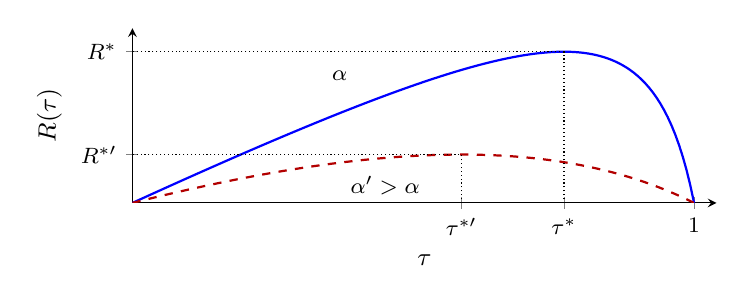
\begin{tikzpicture}
\begin{axis}[width=9cm,height=3.8cm,xmin=0,xmax=1.04,ymin=0,ymax=0.62,axis lines=left,
  xlabel={$\tau$},ylabel={$R(\tau)$},xtick={0.58579,0.76834,1},xticklabels={$\tau^{*\prime}$,$\tau^*$,$1$},
  ytick={0.17157,0.53668},yticklabels={$R^{*\prime}$,$R^*$},tick label style={font=\footnotesize},label style={font=\small}]
\addplot[thick,blue,domain=0:1,samples=150]{x*(1-x)/(1.1-x)};
\addplot[thick,red!70!black,dashed,domain=0:1,samples=150]{x*(1-x)/(2-x)};
\addplot[densely dotted] coordinates {(0.76834,0) (0.76834,0.53668) (0,0.53668)};
\addplot[densely dotted] coordinates {(0.58579,0) (0.58579,0.17157) (0,0.17157)};
\node[font=\footnotesize,anchor=south east] at (axis cs:0.40,0.40) {$\alpha$};
\node[font=\footnotesize,anchor=north] at (axis cs:0.45,0.13) {$\alpha'>\alpha$};
\end{axis}
\end{tikzpicture}
\end{center}
\intuicao{Revenue peaks where the base falls as fast, in percent, as the rate rises: $e_{BB}\,\tau=1-\tau$ (see (d)).}
\refbib{Kurlat (2020), \S7.3 and Exercise 7.5(e).}
\rubrica{
\item $R$, sign of $R'$: 1 pt. Single peak, $\tau^*$, $R^*$: 1 pt. Cap: unproved sign of $R'$, 0 for it.
\item Graph (scored apart): axes, humps, peaks marked, the $\alpha'$ curve lower and peaking left: 1 pt.
}
\end{sol}

\textbf{c)} (3 points) Derive in closed form the welfare cost of the program in consumption-equivalent terms: the share $x(\tau)$ of
consumption at $\tau=0$ the household would give up to avoid the program. Determine its order at $\tau=0$ and its monotonicity in
$\tau$; find its leading term around $\tau=0$ and its limit as $\tau\to1$.
\resolespaco
\begin{sol}
\passo{welfare}{With $c=h$, $U(\tau)=\ln h(\tau)+\alpha\ln(1-h(\tau))$, and $x$ solves $\ln[(1-x)\,c(0)]+\alpha\ln(1-h(0))=U(\tau)$. With $h=\frac{1-\tau}{1+\alpha-\tau}$
and $1-h=\frac{\alpha}{1+\alpha-\tau}$:
\[\ln(1-x)=\ln(1-\tau)+(1+\alpha)\ln\frac{1+\alpha}{1+\alpha-\tau},\qquad x(\tau)=1-(1-\tau)\Big(\frac{1+\alpha}{1+\alpha-\tau}\Big)^{1+\alpha}.\]}
\passo{shape}{$\frac{d}{d\tau}\ln(1-x)=-\frac1{1-\tau}+\frac{1+\alpha}{1+\alpha-\tau}=-\frac{\alpha\tau}{(1-\tau)(1+\alpha-\tau)}$: zero at $\tau=0$ (no first-order cost) and negative on
$(0,1)$, so $x$ is strictly increasing. As $\tau\to1$, $1-\tau\to0$ while the other factor tends to $(\frac{1+\alpha}{\alpha})^{1+\alpha}$: $x\to1$.}
\passo{leading term}{The derivative is $-\frac{\alpha}{1+\alpha}\tau+O(\tau^2)$; integrating from $\ln(1-x(0))=0$, $x(\tau)=\frac{\alpha}{1+\alpha}\,\frac{\tau^2}{2}+O(\tau^3)$:
Harberger's triangle $\frac12e_H\tau^2$, with $e_H=\frac{\alpha}{1+\alpha}$ the Hicksian elasticity at $\tau=0$ (see (d)).}
\intuicao{The program moves nothing between identical households; its whole effect is the wedge on the price of leisure, a pure
substitution effect, second order near zero.}
\refbib{Kurlat (2020), Exercise 7.5(g)--(h).}
\rubrica{
\item Closed form: 1 pt. First-order zero, monotonicity, limit, proved: 1 pt. Leading term, $e_H$: 1 pt.
\item Caps: unproved sign or limit, 0 for it; revenue thrown away (one model only), max.\ half.
}
\end{sol}

\textbf{d)} (3 points) At the balanced-budget allocation, for $\tau\in(0,1)$, derive the Marshallian and Hicksian elasticities of individual hours
with respect to the after-tax wage $w_n=1-\tau$, the balanced-budget elasticity $e_{BB}\equiv d\ln h/d\ln(1-\tau)$, and the Frisch elasticity.
Order the four for every $\tau\in(0,1)$ and say which one Prescott's experiment uses.
\resolespaco
\begin{sol}
\passo{Marshallian}{From (a) with $w_n$ free, $h=\frac1{1+\alpha}-\frac{\alpha T}{(1+\alpha)w_n}$: $h_w\equiv\frac{\partial h}{\partial w_n}=\frac{\alpha T}{(1+\alpha)w_n^2}$, $h_T\equiv\frac{\partial h}{\partial T}=-\frac{\alpha}{(1+\alpha)w_n}$.
At $T=\tau h$, $w_n=1-\tau$: $e_M=\frac{w_nh_w}{h}=\frac{\alpha\tau}{(1+\alpha)(1-\tau)}$.}
\passo{Hicksian}{Slutsky (the compensating transfer moves by $-h\,dw_n$): $\frac{\partial h^H}{\partial w_n}=h_w-h\,h_T=\frac{\alpha(T+w_nh)}{(1+\alpha)w_n^2}=\frac{\alpha c}{(1+\alpha)w_n^2}$;
with $c=h$, $e_H=\frac{\alpha}{(1+\alpha)(1-\tau)}$.}
\passo{balanced budget and Frisch}{$\ln h(\tau)=\ln(1-\tau)-\ln(1+\alpha-\tau)$ gives $e_{BB}=1-h=\frac{\alpha}{1+\alpha-\tau}$. With the marginal utility of
wealth $\lambda$ fixed, $\frac{\alpha}{1-h}=\lambda w_n$ gives $\frac{dh}{d\ln w_n}=1-h$: $e_F=\frac{1-h}{h}=\frac{\alpha}{1-\tau}$.}
\passo{ordering}{$e_F=(1+\alpha)e_H>e_H>\tau e_H=e_M$; $e_H-e_{BB}=\frac{\alpha^2\tau}{(1+\alpha)(1-\tau)(1+\alpha-\tau)}>0$; and
$e_{BB}-e_M=\frac{\alpha\,N(\tau)}{(1+\alpha)(1-\tau)(1+\alpha-\tau)}$, with $N$ from (b), so $e_{BB}\gtrless e_M$ iff $\tau\lessgtr\tau^*$. Why: $h'(\tau)=-h_w+h_TR'(\tau)$, so $e_{BB}=e_M+\frac{1-\tau}{h}\,|h_T|\,R'(\tau)$: below the peak a tax cut also cuts the transfer, an income
effect that adds to the wage effect. So $e_F>e_H>e_{BB}>e_M$ for $\tau<\tau^*$; above $\tau^*$, $e_{BB}<e_M$.}
\passo{which one}{Prescott compares economies whose revenue is rebated: his experiment uses $e_{BB}$, and $R'(\tau^*)=0$ reads
$\tau^*=1/[1+e_{BB}(\tau^*)]$. Kurlat's Exercise 7.5(j)--(l) computes $e_F$ to compare it with micro estimates.}
\intuicao{They hold different things fixed: the transfer ($e_M$), utility ($e_H$), the budget ($e_{BB}$), the marginal utility of wealth
($e_F$); only $e_{BB}$ lets the transfer move, so only its rank depends on the side of the peak.}
\refbib{Kurlat (2020), \S7.3 and Exercise 7.5(j)--(l).}
\rubrica{
\item Each elasticity: 0.5 pt (2 pts). Ordering, threshold $\tau^*$ proved, Prescott's choice: 1 pt.
\item Cap: elasticities at a single $\tau$ (special case for the general one), max.\ half.
}
\end{sol}

\textbf{e)} (3 points) \emph{Parameter analysis.} Sign the effects of $\alpha$ and of $\tau$ on $h$, $R$, $\tau^*$, $R^*$, $x$ and $e_{BB}$, prove each sign and
collect them in a table. Find the limits as $\alpha\to0$ and $\alpha\to\infty$ and a bound on $\tau^*$ valid for every $\alpha$, and read the results.
\resolespaco
\begin{sol}
\passo{direct signs}{$\frac{\partial h}{\partial\alpha}=-\frac{1-\tau}{(1+\alpha-\tau)^2}<0$, $h'(\tau)<0$ (a); $\frac{\partial R}{\partial\alpha}<0$, $R'$ has the sign of $N(\tau)$ (b);
$\frac{\partial e_{BB}}{\partial\alpha}=\frac{1-\tau}{(1+\alpha-\tau)^2}>0$, $\frac{\partial e_{BB}}{\partial\tau}=\frac{\alpha}{(1+\alpha-\tau)^2}>0$; $\frac{\partial x}{\partial\tau}>0$ (c).}
\passo{Laffer peak}{$\frac{d\tau^*}{d\alpha}=1-\frac{1+2\alpha}{2\sqrt{\alpha(1+\alpha)}}<0$ because $(1+2\alpha)^2=4\alpha(1+\alpha)+1$; $R^*=(\sqrt{1+\alpha}+\sqrt\alpha)^{-2}$ falls with $\alpha$.}
\passo{welfare cost}{With $a\equiv1+\alpha$, $\ln(1-x)=\ln(1-\tau)+a\ln\frac{a}{a-\tau}$ and $\frac{\partial}{\partial a}\big[a\ln\frac{a}{a-\tau}\big]=\ln(1+z)-z<0$ for $z\equiv\frac{\tau}{a-\tau}>0$
($\ln(1+z)-z$ is $0$ at $z=0$ with derivative $-\frac{z}{1+z}$): $x$ rises with $\alpha$.}
\par\smallskip{\centering\begin{tabular}{lcc}
\toprule
 & $\partial/\partial\alpha$ & $\partial/\partial\tau$ \\
\midrule
hours $h(\tau)$ & $-$ & $-$ \\
revenue $R(\tau)$ & $-$ & $+$ iff $\tau<\tau^*$ \\
Laffer peak $\tau^*$, largest program $R^*$ & $-$ & $0$ \\
welfare cost $x(\tau)$ & $+$ & $+$ \\
elasticity $e_{BB}$ & $+$ & $+$ \\
\bottomrule
\end{tabular}\par}
\passo{limits and bound}{$\alpha\to0$: $\tau^*\to1$, $R^*\to1$, $h\to1$, $x\to0$, $e_{BB}\to0$. $\alpha\to\infty$: $\sqrt{\alpha^2+\alpha}=\alpha+\frac12-\frac1{8\alpha}+O(\alpha^{-2})$ gives
$\tau^*\downarrow\frac12$; $R^*\sim\frac1{4\alpha}$, $h\to0$, $e_{BB}\to1$, and $a\ln\frac{a}{a-\tau}\to\tau$ gives $x\to1-(1-\tau)e^{\tau}$, a bound on the cost for every $\alpha$.
As $(\alpha+\frac12)^2-\alpha(1+\alpha)=\frac14$, $\tau^*\in(\frac12,1)$ for every $\alpha$. Knife-edges: $\tau=0$ (no first-order cost, $e_{BB}=e_H$); $\tau^*$ ($e_{BB}=e_M$).}
\passo{reading}{A larger $\alpha$ makes hours more responsive: the base shrinks faster, the peak comes earlier (never below one half),
the largest program shrinks and each rate costs more welfare; as $\alpha\to0$ the tax is lump-sum. Prescott's account of Europe's lower
hours needs a large $\alpha$, an $e_{BB}$ at the top of the micro estimates (Kurlat \S7.3).}
\refbib{Kurlat (2020), \S7.3 and Exercise 7.5.}
\rubrica{
\item Signs, including $d\tau^*/d\alpha$ and $\partial x/\partial\alpha$, proved: 1.5. Table, limits, reading: 0.5 each.
\item Caps: a sign without proof, 0 for it; analysis without proofs or reading, max.\ half.
}
\end{sol}
